% !TEX TS-program = lualatex
% !TEX encoding = UTF-8

% This is a simple template for a LuaLaTeX document using gregorio scores.

\documentclass[letterpaper,12pt]{book} % use larger type; default would be 10pt

\input{header.inc}

\geometry{letterpaper,outer=0.4in,inner=0.9in,top=0.5in,bottom=0.6in}

\begin{document}
\garamondbig
\greannotation{Hymn.}
\greannotation{1.}
\gregorioscore{173_hy--auctor_beate_saeculi--solesmes}

\bigskip

\begin{centering}

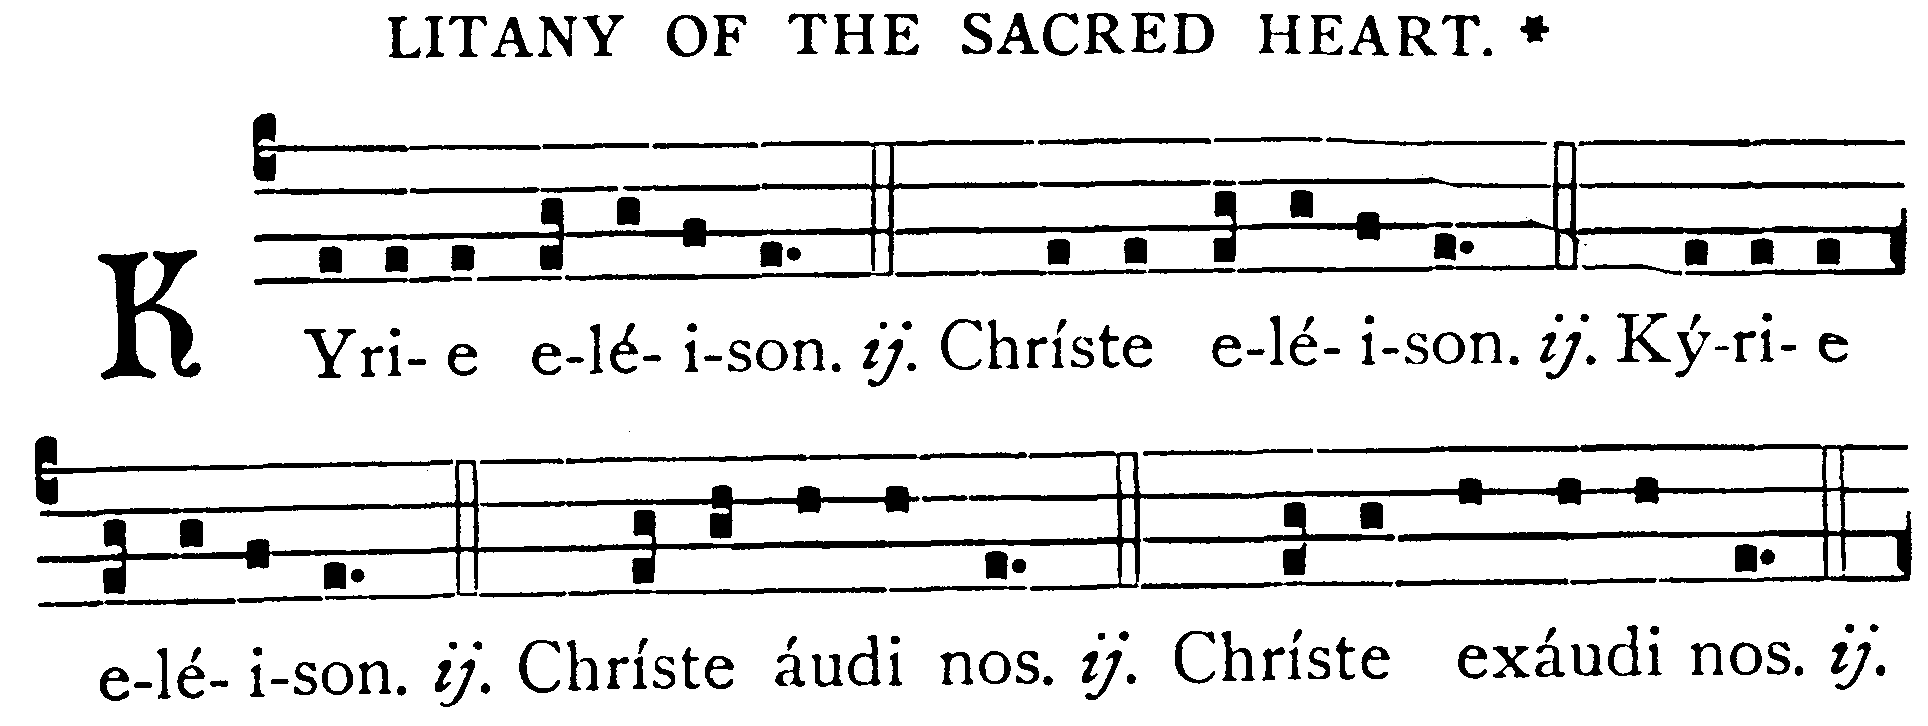
\includegraphics[width=0.98\textwidth]{175-1.png}
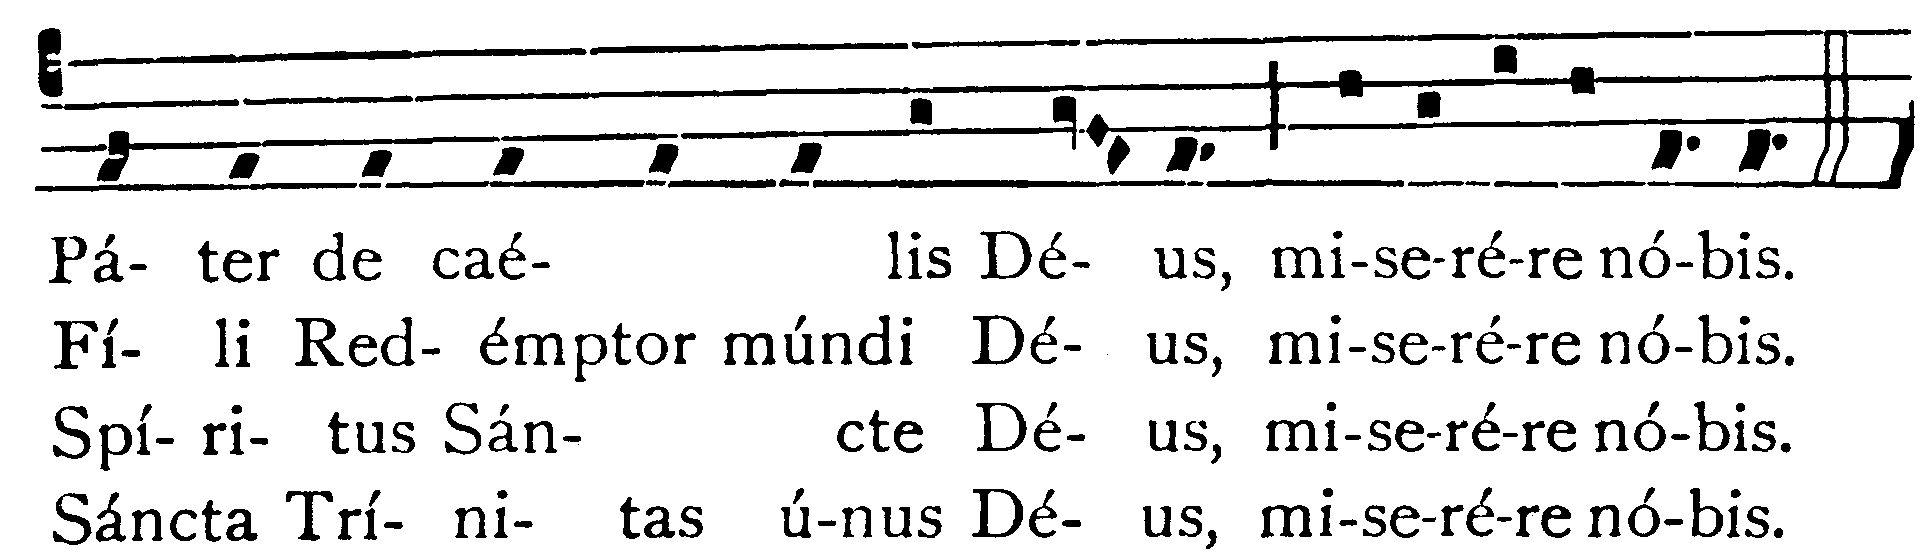
\includegraphics[width=0.98\textwidth]{175-2.png}
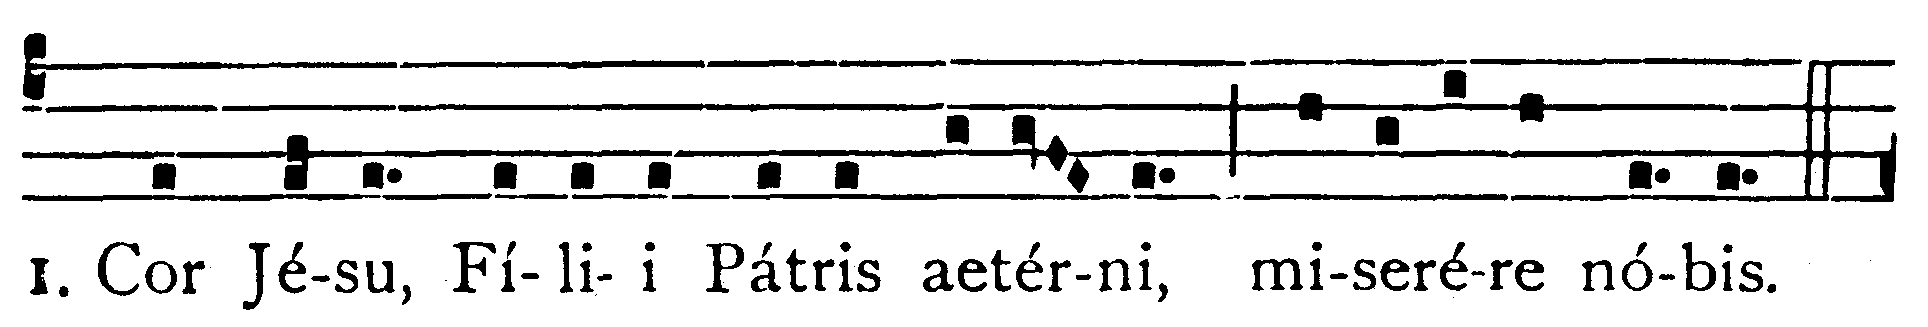
\includegraphics[width=0.925\textwidth]{175-3.png}

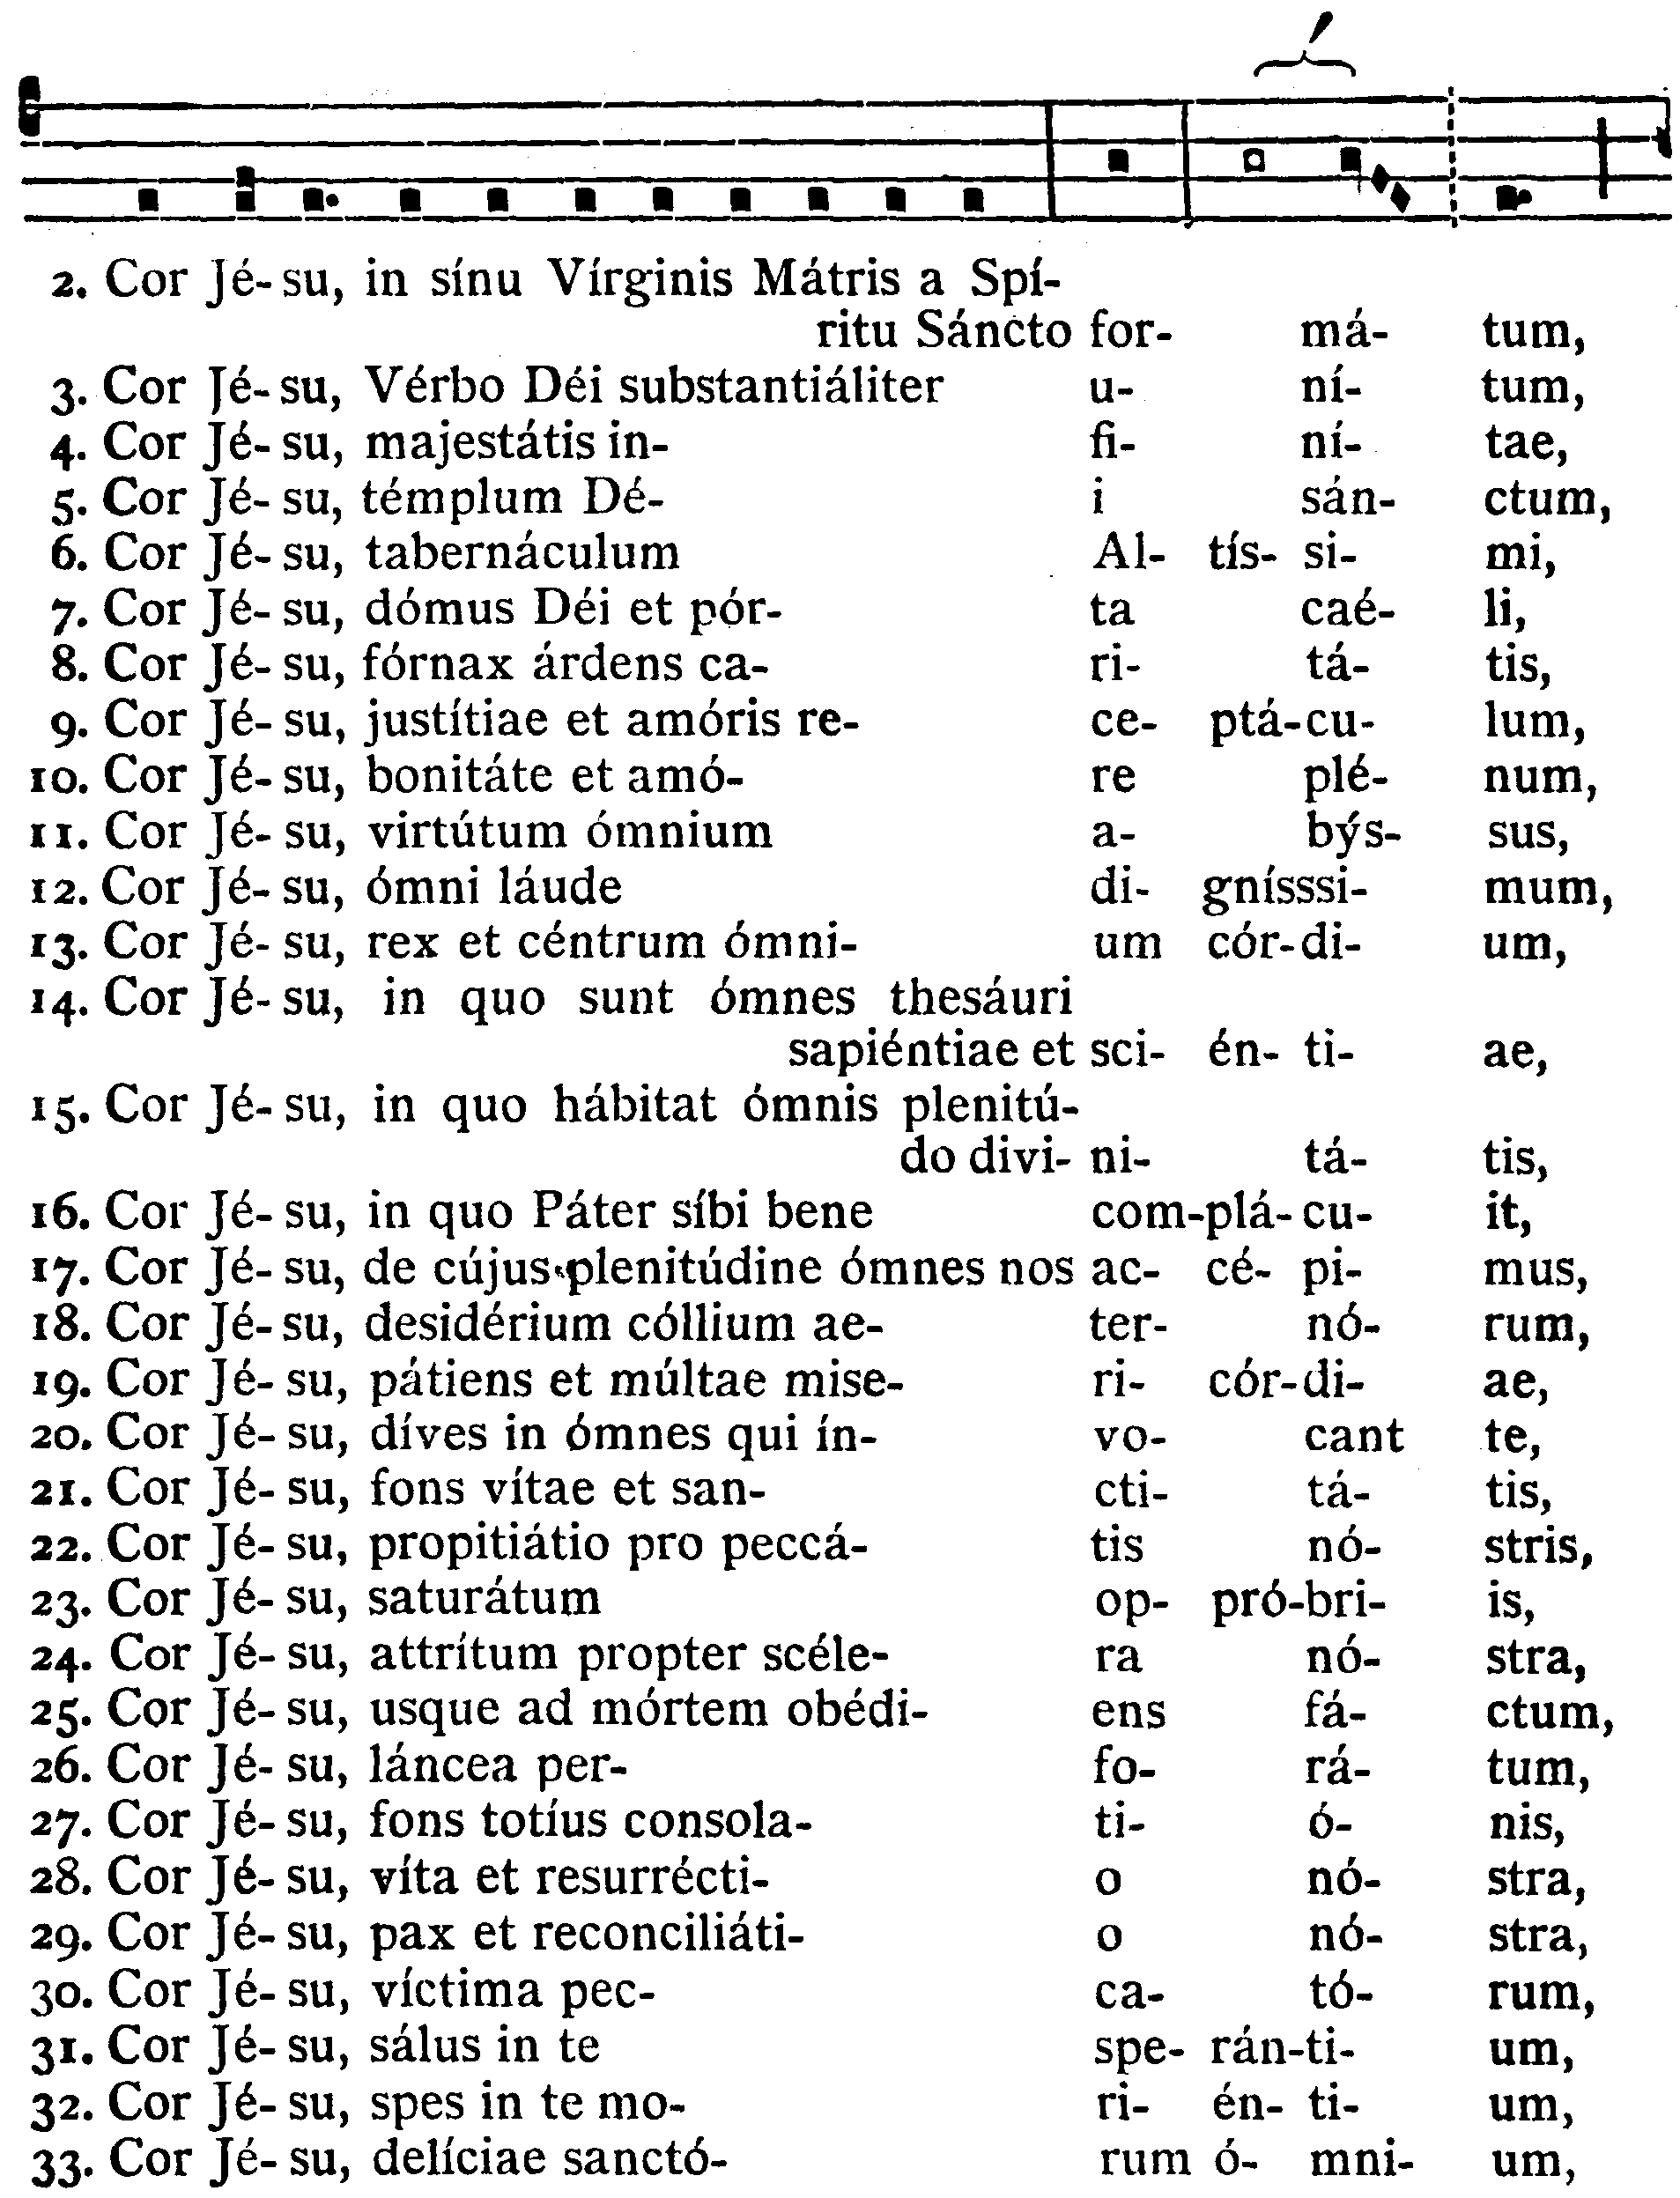
\includegraphics[width=0.925\textwidth]{175-4.png}
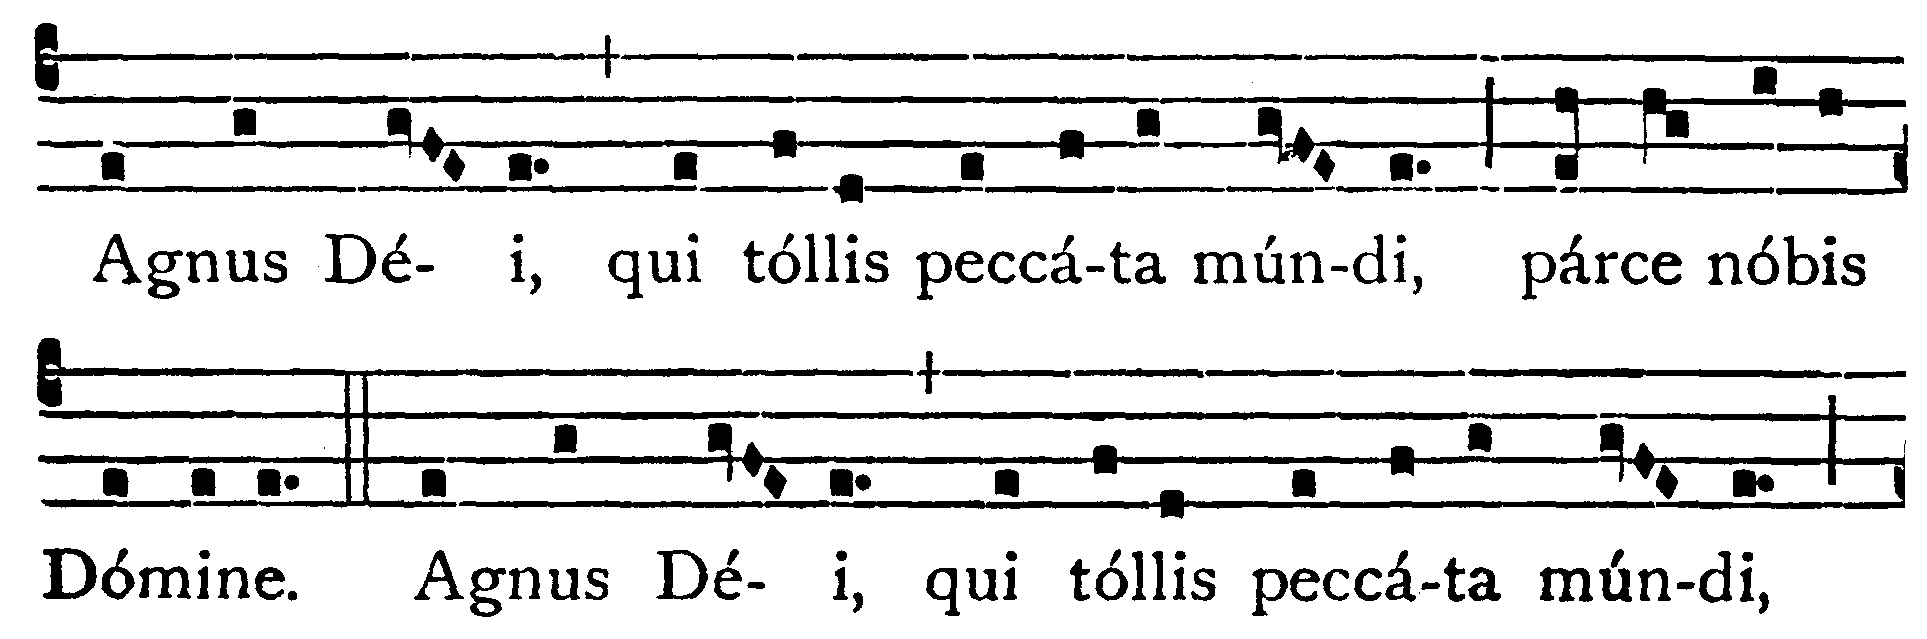
\includegraphics[width=\textwidth]{175-5.png}

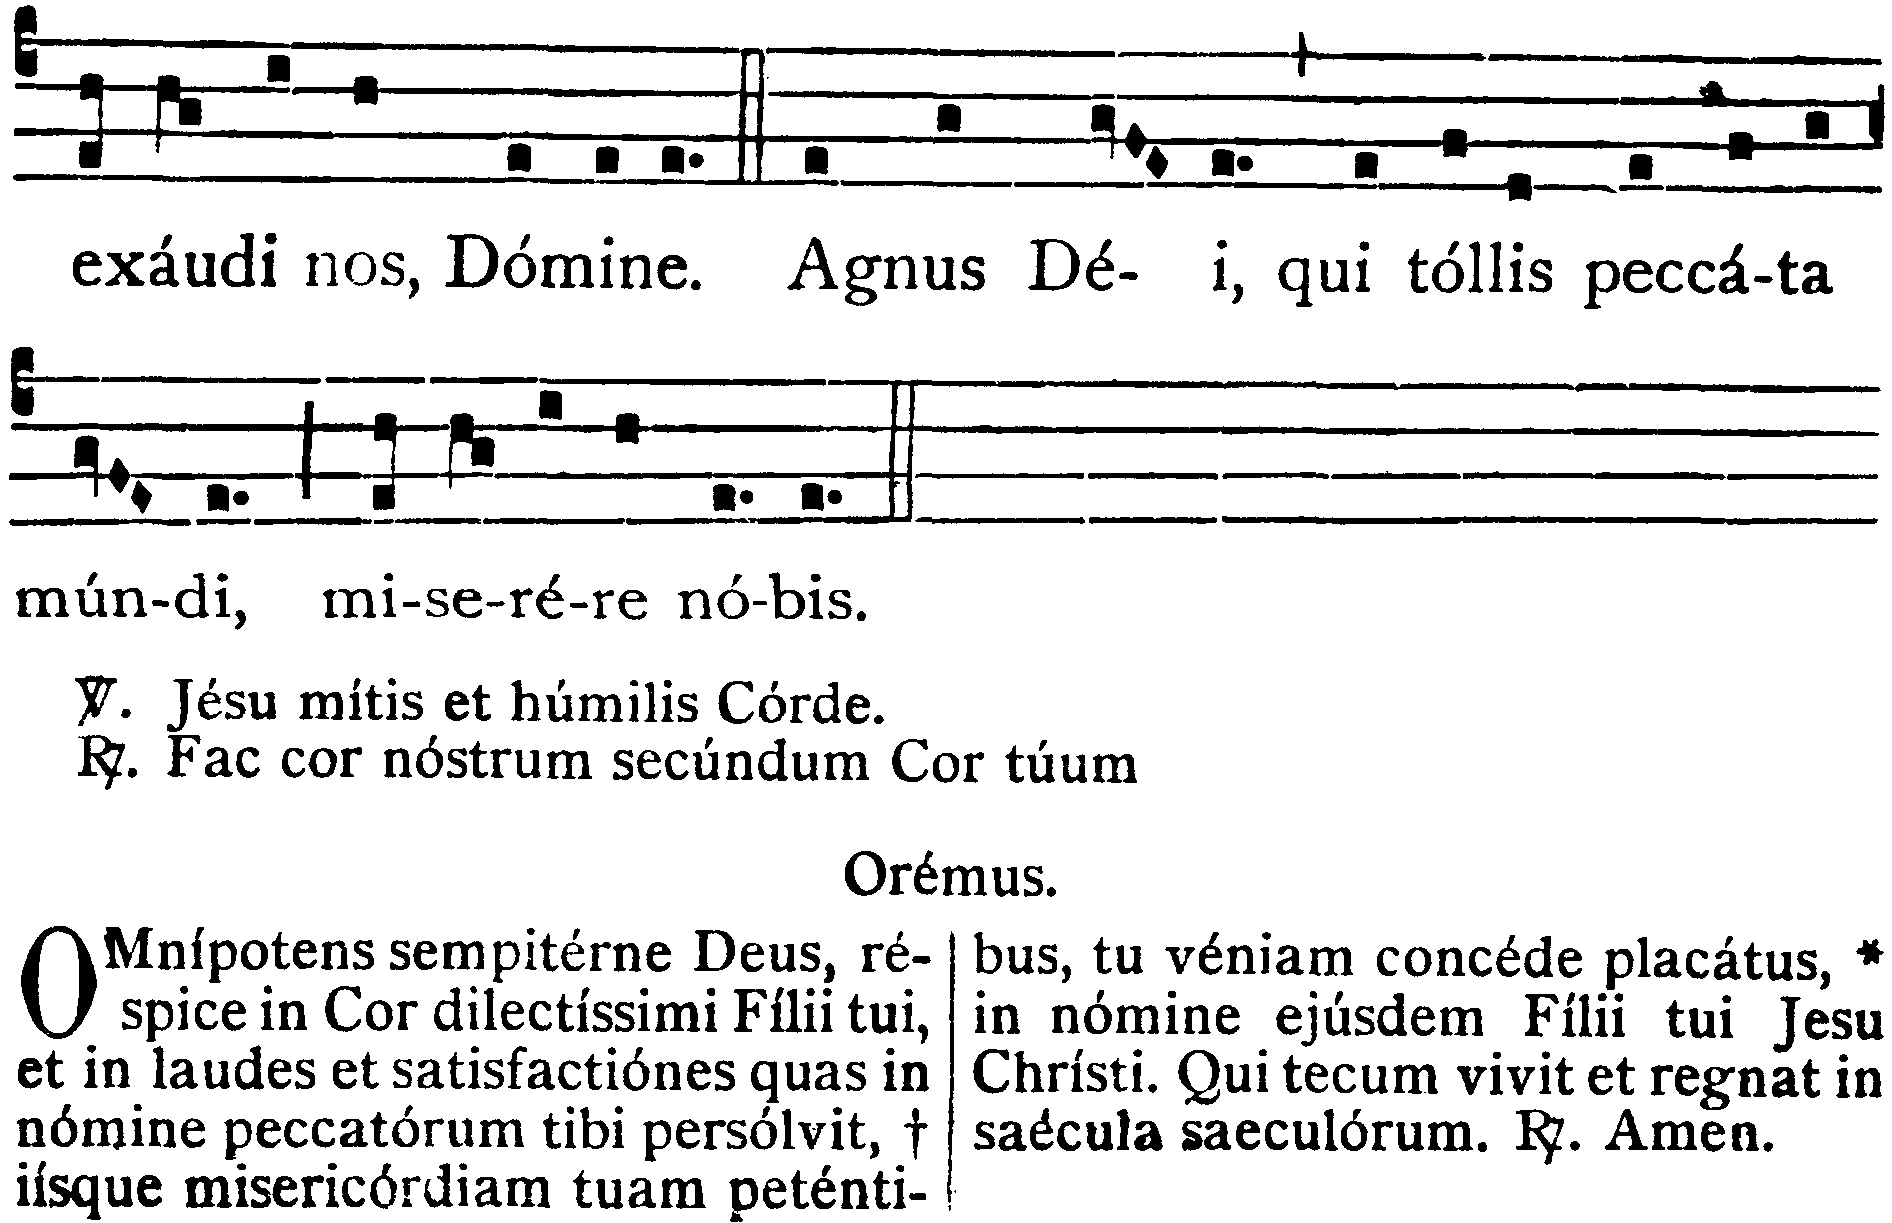
\includegraphics[width=\textwidth]{175-6.png}

\bigskip

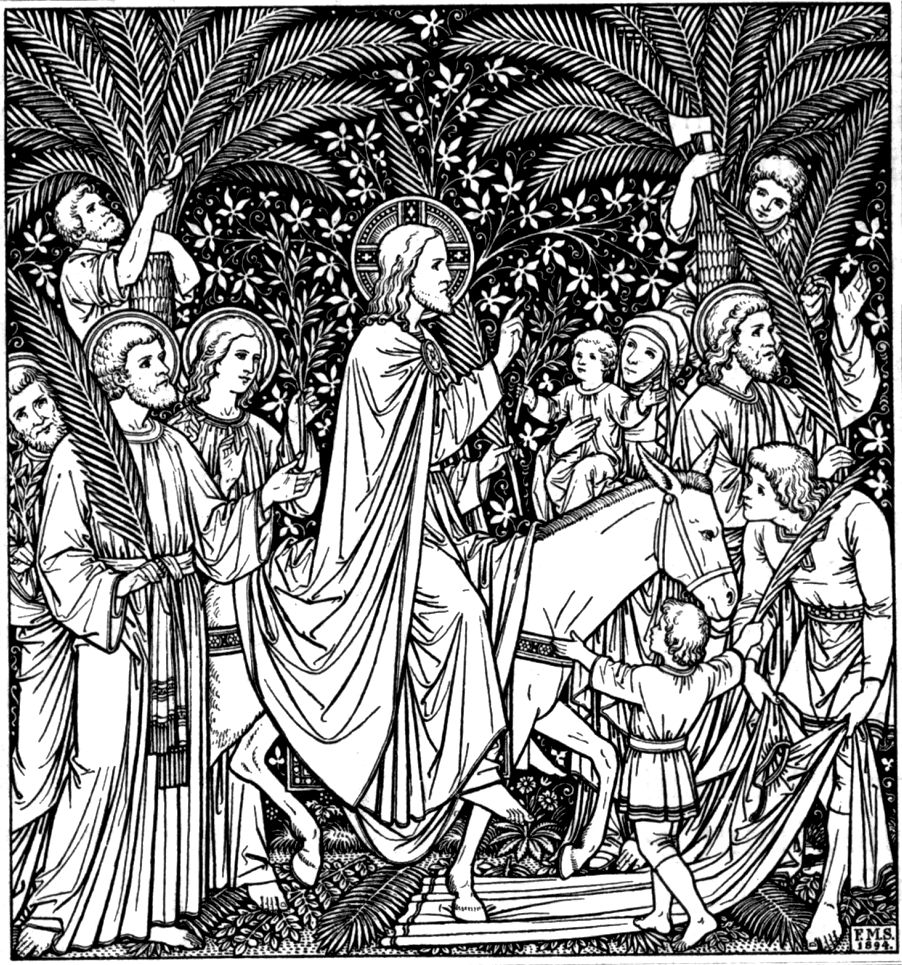
\includegraphics[width=0.35\textwidth]{../177_clipart.png}

\end{centering}

\end{document}